\section{离线神经块均衡器}

\subsection{网络结构与输入输出}

网络输入为接收帧 $y_{0:1023}$ 与已知符号掩码：掩码只在 Adapt Pilot 位置填入已知 Pilot 符号，其余位置置零。这样网络在推理时看不到任何 Data 真值，只看到当前帧的合法 Pilot 与接收波形。网络采用 4 层迭代展开结构，隐藏维度 $d_{\mathrm{model}}=64$，4 个注意力头，配置记录为 Adapter/LoRA rank 8，并在每帧执行 8 次物理 warm start。输出层产生 1024 个 logits。整个网络含 189,350 个参数。图 1 给出结构与训练流程。网络输出的是 logits 而不是硬判决；soft 输出既用于最终 BER 评分前的符号判决，也用于在线 Data 后验，同一组 logits 在两个阶段保持相同语义，避免训练与部署之间的接口漂移。

\begin{figure}[htbp]
\centering
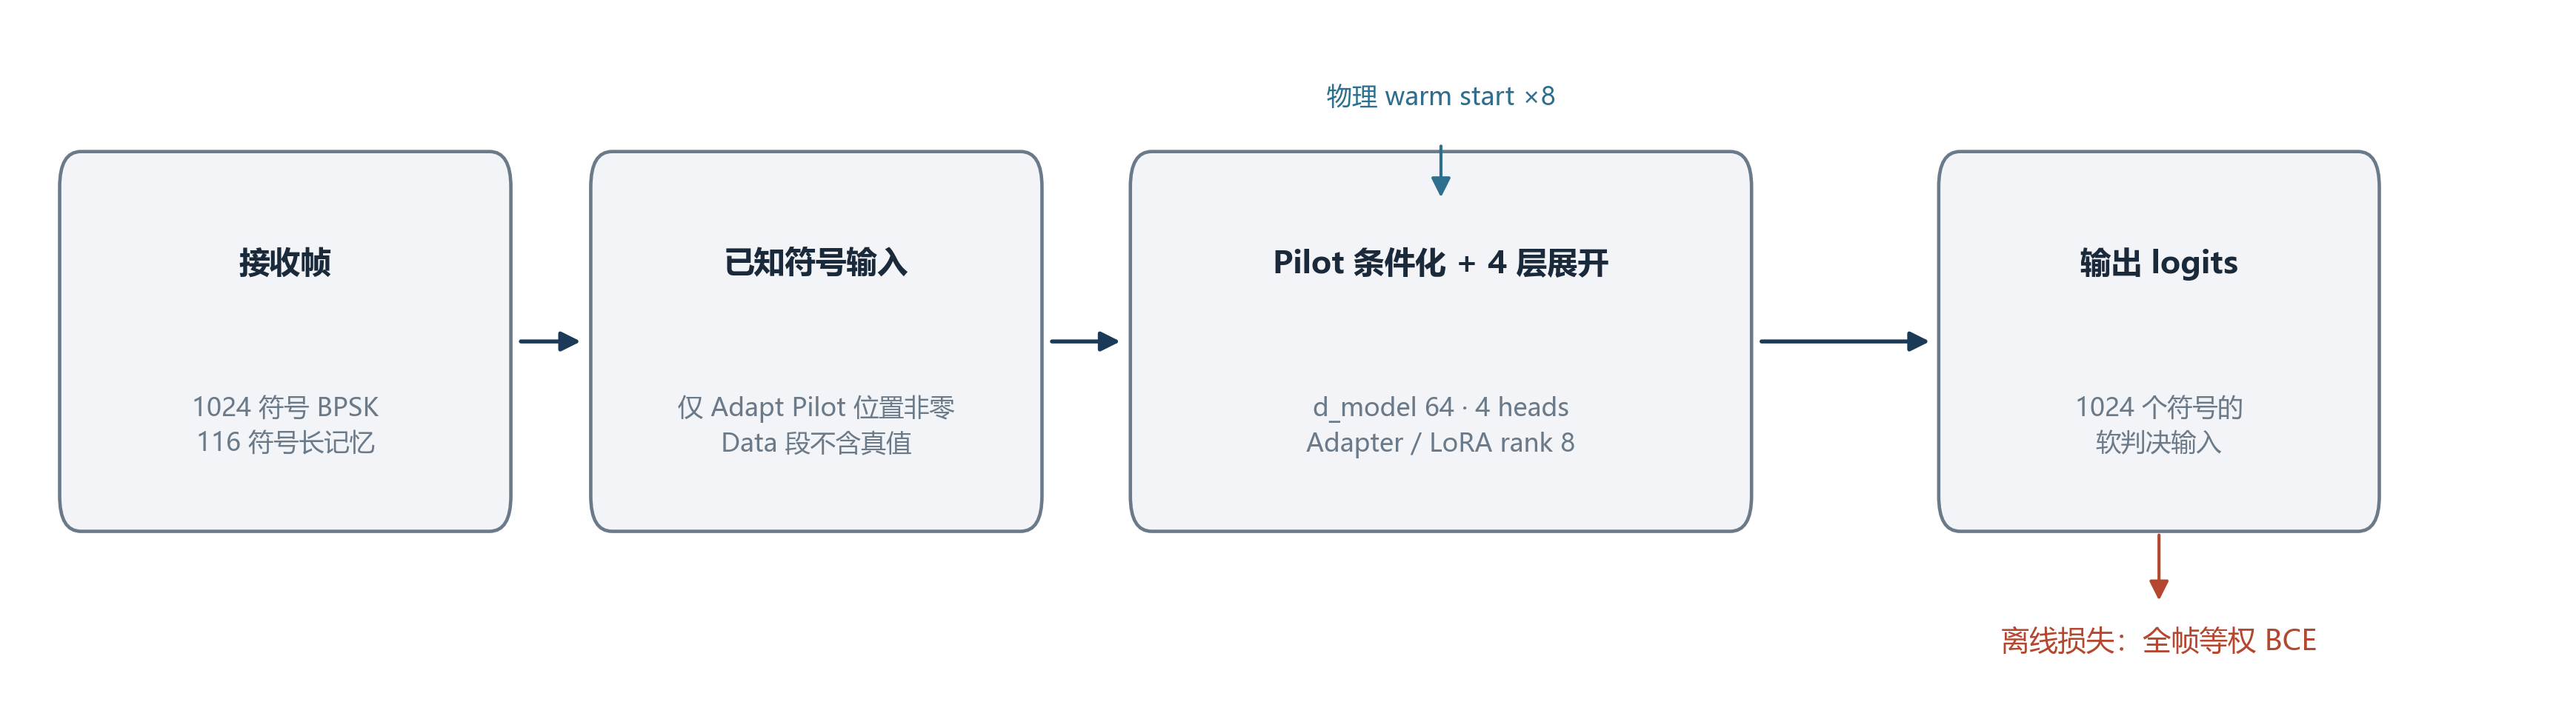
\includegraphics[width=0.95\linewidth]{figures/fig_offline_arch.png}
\caption{离线神经块均衡器的结构与训练流程。接收帧与仅在 Adapt Pilot 位置非零的已知符号输入共同进入 Pilot 条件化的 4 层展开网络；网络输出 1024 个符号的 logits，离线以全帧等权 BCE 训练。}
\end{figure}

展开结构的作用是把“信道估计—均衡—判决”的迭代过程变成可学习的层间映射：物理模型提供先验，网络学习难以手工建模的残差。Pilot 条件化使同一组权重可以根据当前帧的 Pilot 观测调整输出，而不需要在部署时更新权重。与把整个接收机视为黑箱的做法相比，展开结构保留了 116 符号长记忆的物理先验，使离线样本需求可控；与纯模型驱动方法相比，它又能从仿真标签中学习难以手工建模的残差。

\subsection{离线训练目标与数据角色}

离线损失为全帧等权二元交叉熵：

\begin{equation*}
\mathcal{L}_{\mathrm{BCE}}=\frac{1}{T}\sum_{t=1}^{T}\left[-b_t\log\sigma(z_t)-(1-b_t)\log(1-\sigma(z_t))\right],
\end{equation*}

其中 $b_t$ 为发送比特，$\sigma(\cdot)$ 为 sigmoid，$T=1024$。训练使用仿真信道生成的接收帧与完整标签，batch size 为 1，共 32 步；训练日志记录 32 个 \texttt{estimated\_cir\_level\_b} 更新步，条件 CIR 来源为 acquisition。checkpoint 的选择指标是独立验证切片的 Data BER，而不是 Pilot BCE。用 Data BER 而不是 Pilot BCE 选择 checkpoint，是为了让离线模型的选择目标与最终指标一致。Pilot BCE 只反映已知符号的拟合，不能代表 Data 段泛化；在长记忆信道中，Pilot 段与 Data 段的残余信道状态不同，若按 Pilot BCE 选择，容易得到在 Pilot 上过拟合、在 Data 上退化的模型。源 checkpoint 的 SHA256 为 \texttt{8cd3912d1c957c9689c51730aff9d27a8f74942186c802a7483e5781af65aec4}，元数据记录 \texttt{resume\_loaded=False}、189,350 参数、\texttt{iterations=4}、\texttt{d\_model=64}、\texttt{physics\_warm\_start\_iterations=8}，离线验证 \texttt{mean\_ber\_data $\approx$ 0.0658}。

需要说明复现边界：原始训练命令、源码 revision、Python/PyTorch/CUDA 环境、完整优化器超参数与显式随机种子没有随 checkpoint 保存。本文给出的训练配置来自配置文件和训练指标的重构，不能称为严格复现。离线主矩阵的结论主要由独立评估支撑，而不是由 4 帧内部验证集单独支撑。

\subsection{离线饱和与可修复空间}

在进入在线设计前，本文先判断离线模型是否已经饱和。在 3 seed × 12 帧的配对评估中，从同一 checkpoint 继续训练 32/64 步，或在相同 32 步预算下把 \texttt{iterations} 从 4 增到 6、\texttt{d\_model} 从 64 增到 96，Frozen Data BER 与原始 checkpoint 基本重合；最大点估计改善仅约 $-1.8\times10^{-4}$（5 dB，64 步续训），对应 12 帧约 1–2 个比特，其余点多数量级为 0 或区间跨零。增加训练步数或模型宽度没有带来可确认的改善。

另一方面，在 5 seed × 8 帧的 oracle 诊断中（seed 91001–91005），把条件 CIR 换成该帧真实 CIR 后，Frozen BER 在 5 dB 从 0.05283 降到 0.04199（$\Delta=-1.08\times10^{-2}$，95\% CI $[-1.57\times10^{-2},-5.94\times10^{-3}]$），10 dB 从 0.00700 降到 0.00465（$\Delta=-2.34\times10^{-3}$，CI $[-3.23\times10^{-3},-1.46\times10^{-3}]$）；0 dB 点估计为 $-4.60\times10^{-2}$，5/5 seed 同向，但 seed 91003 的 BER 0.311 使区间跨零；15 dB 近似为 0。这个 oracle 分支不可部署，只用于诊断：它说明 5/10 dB 的剩余误差主要来自 CIR 估计，而不是网络容量或训练预算。在线适配因此应优先作用于物理状态，而不是继续扩大神经模型。这一诊断也解释了为什么本文优先选择在线 CIR 后验，而不是继续增加同分布训练样本：如果剩余误差主要来自 CIR 估计，那么增加同分布训练样本只能改善网络对已有条件的拟合，不能纠正部署时的信道失配。相反，在线 CIR 后验直接作用于失配的来源，且不需要 Data 标签。该判断只适用于本文的 116 符号长回波配置与当前 checkpoint；在其他信道或模型上，误差构成可能不同，需重新做 oracle 诊断。
